\documentclass{article}
\usepackage[utf8x]{inputenc}
\usepackage[english,russian]{babel}
\usepackage{graphicx}
\usepackage{hyperref}
\begin{document}
\title{Тестирование алгоритма миграции Кирхгофа на точечном источнике}
\author{\textbf{м.н.с. Голубев В.И.} \\ Лаборатория прикладной вычислительной геофизики МФТИ}
\maketitle

Мною был реализован алгоритм миграции на основе вычисления интеграла Рэлея (формула 15.208 из книги).
В качестве тестового расчёта использована синтетическая сейсмограмма, полученная от точечного (по пространству) источника со временной функцией
вида Ricker wavelet (\url{http://subsurfwiki.org/wiki/Ricker_wavelet}). Она получена аналитически в лучевом приближении распространения возмущения:
\begin{equation}
\label{eq_seismogram_ricker}
U(\vec{r}, t) = \frac{1}{4\pi d}(1 - 2\pi^2f^2t^2_d)\exp(-\pi^2f^2t^2_d),
\end{equation}
где $d(\vec{r})$ - расстояние от точки расположения источника до точки расположения сейсмоприёмника, а $t_d(\vec{r}) = t - \frac{d}{c}$ - время с учётом распространения сигнала вдоль прямой.
Частота сигнала $f$ равнялась 50 Гц.
Синтетическая сейсмограмма приведена на рис. (\ref{img_seismogram_ricker}).
\begin{figure}[ht]
  \center
  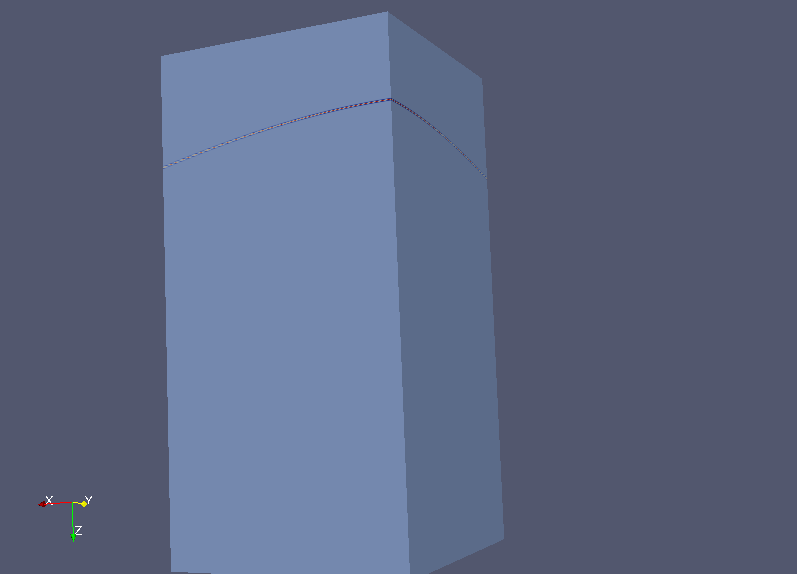
\includegraphics[scale=0.5]{pic/point_source_input_1000_1000_1000.png}
  \caption{Синтетическая сейсмограмма (ось Z - ось времени). Источник точечный (Ricker 50 Hz), находится в самом центре области (куб со стороной 2000)  в точке 1000, 1000, 1000.}
\label{img_seismogram_ricker}
\end{figure}
Согласно общей идее после миграции должно получиться точное местоположение источника. Мигрированное изображение приведено на рис. (\ref{img_migrated_ricker}).
Идея с использованием Ricker wavelet взята с \url{http://utam.gg.utah.edu/UTAMtheses/HongchuanSun/html/node13.html}. Кстати, там вроде бы опечатка и $c$ не 5000 м/с, а 2500 м/с.
\begin{figure}[ht]
  \center
  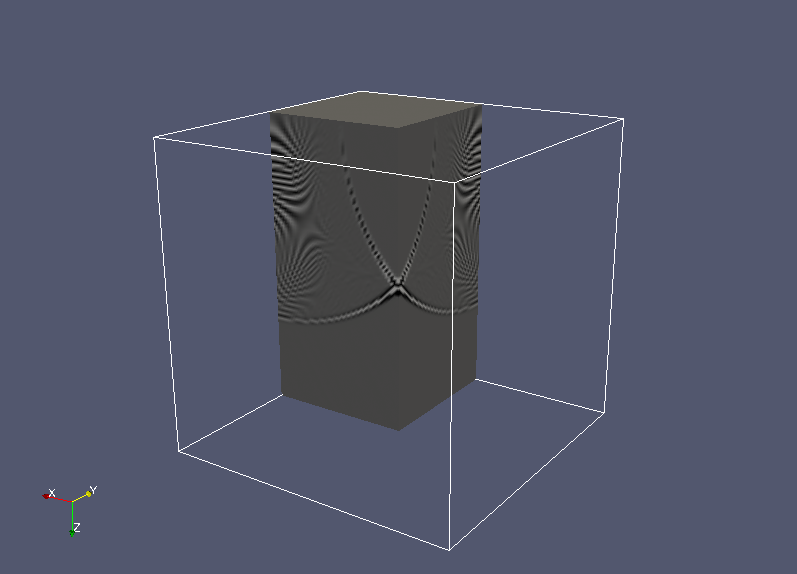
\includegraphics[scale=0.5]{pic/point_source_output_1000_1000_1000.png}
  \caption{Мигрированное изображение точечного источника, расположенного точно в центре области. Источник точечный (Ricker 50 Hz). Сделано сечение плоскостями $OXZ$ и $OYZ$.}
\label{img_migrated_ricker}
\end{figure}

\end{document}
